\documentclass{article}
\usepackage[a4paper, margin=1.5cm]{geometry}
\usepackage[utf8]{inputenc}
\usepackage{amsmath,amssymb}
\usepackage{amsthm}
\usepackage{tikz}
\usetikzlibrary{automata,arrows,positioning}

\title{INT201 Assignment 1}
\author{Xinrong Li (ID: 2363123)}
\date{}

\newtheorem{theorem}{Theorem}

\begin{document}
\maketitle

\section{DFA for Strings Starting with \texttt{b} and Ending with \texttt{a}}
We construct a deterministic finite automaton (DFA) for the language
\[
L_1 = \{\,x \in \{a,b\}^* \mid x \text{ starts with ``b'' and ends with ``a''}\}\,.
\]
Recall that a DFA is formally defined as a 5-tuple $(Q, \Sigma, \delta, q_0, F)$, where $Q$ is a finite set of states, $\Sigma$ is the input alphabet, $\delta: Q\times \Sigma \to Q$ is the transition function, $q_0 \in Q$ is the initial state, and $F \subseteq Q$ is the set of accepting states.

\medskip

\noindent \textbf{DFA Construction:}
Let $M_1 = (Q, \Sigma, \delta, q_0, F)$ with:
\begin{itemize}\itemsep0em
    \item $Q = \{q_0, q_1, q_2, q_d\}$, where $q_0$ is the start state and $q_d$ is a dead (sink) state.
    \item $\Sigma = \{a, b\}$.
    \item Transition function $\delta$ defined as:
          \[
          \begin{aligned}
          \delta(q_0, a) &= q_d, & \delta(q_0, b) &= q_1,\\
          \delta(q_1, a) &= q_2, & \delta(q_1, b) &= q_1,\\
          \delta(q_2, a) &= q_2, & \delta(q_2, b) &= q_1,\\
          \delta(q_d, a) &= q_d, & \delta(q_d, b) &= q_d~,
          \end{aligned}
          \]
          where $q_d$ is a non-accepting sink that traps any string that does not meet the criteria.
    \item $q_0$ is the initial state.
    \item $F = \{q_2\}$, since $q_2$ represents having read a string that ends in \texttt{a} (and by construction also started with \texttt{b}).
\end{itemize}
Intuitively, $q_1$ signifies that the string read so far starts with \texttt{b} and the last symbol read was \texttt{b}, whereas $q_2$ signifies the string starts with \texttt{b} and the last symbol read was \texttt{a}. The state $q_2$ is accepting, ensuring the input ends in \texttt{a}. Any input that either fails to start with \texttt{b} or cannot end in \texttt{a} (e.g.\ it ended in \texttt{b}) will eventually reach the sink $q_d$ and be rejected.

\begin{figure}[h]\centering
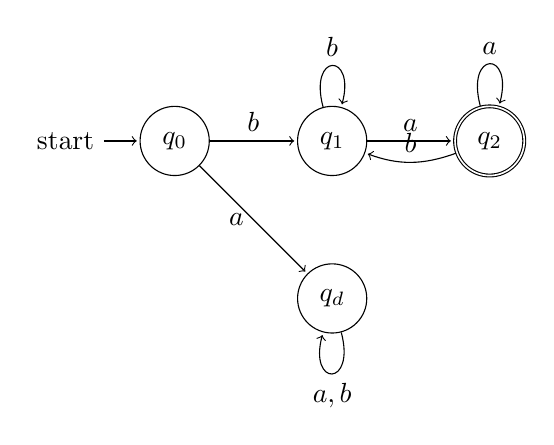
\begin{tikzpicture}[shorten >=1pt,node distance=2cm,on grid,auto]
    \node[state, initial] (q0) {$q_0$};
    \node[state, right=of q0] (q1) {$q_1$};
    \node[state, accepting, right=of q1] (q2) {$q_2$};
    \node[state, below=of q1] (qd) {$q_d$};
    \draw[->] (q0) edge node[above] {$b$} (q1);
    \draw[->] (q0) edge node[left] {$a$} (qd);
    \draw[->] (q1) edge node[above] {$a$} (q2);
    \draw[->] (q1) edge[loop above] node {$b$} ();
    \draw[->] (q2) edge[loop above] node {$a$} ();
    \draw[->] (q2) edge[bend left=20] node[above] {$b$} (q1);
    \draw[->] (qd) edge[loop below] node {$a,b$} ();
\end{tikzpicture}
\caption{DFA $M_1$ for all strings over $\{a,b\}$ that start with \texttt{b} and end with \texttt{a}.}
\end{figure}

\section{Converting an NFA to an Equivalent DFA}
We convert the following NFA over $\Sigma=\{a,b,c\}$ to an equivalent DFA via the subset construction. The NFA has states $Q=\{q_0,q_1,q_2\}$, start state $q_0$, and accepting state $q_2$, with transitions:
\[
q_0 \xrightarrow{\varepsilon} q_1,\quad
q_1 \xrightarrow{\varepsilon} q_2,\quad
q_0 \xrightarrow{a} q_0,\quad
q_1 \xrightarrow{b} q_1,\quad
q_2 \xrightarrow{c} q_2.
\]
Its diagram is shown in Figure~\ref{fig:nfa}.

\begin{figure}[h]\centering
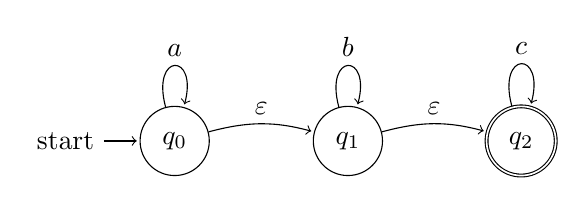
\begin{tikzpicture}[shorten >=1pt,node distance=2.2cm,on grid,auto]
  \node[state, initial]                 (q0) {$q_0$};
  \node[state, right=of q0]             (q1) {$q_1$};
  \node[state, accepting, right=of q1]  (q2) {$q_2$};

  \draw[->] (q0) edge[bend left=15] node[above] {$\varepsilon$} (q1);
  \draw[->] (q1) edge[bend left=15] node[above] {$\varepsilon$} (q2);

  \draw[->] (q0) edge[loop above] node {$a$} ();
  \draw[->] (q1) edge[loop above] node {$b$} ();
  \draw[->] (q2) edge[loop above] node {$c$} ();
\end{tikzpicture}
\caption{NFA $M_2$ used in Question 2.}
\label{fig:nfa}
\end{figure}

\noindent\textbf{Subset construction (concise).}
The $\varepsilon$-closures are
\[
\varepsilon\text{-closure}(q_0)=\{q_0,q_1,q_2\},\quad
\varepsilon\text{-closure}(q_1)=\{q_1,q_2\},\quad
\varepsilon\text{-closure}(q_2)=\{q_2\}.
\]
Thus the reachable DFA states (as subsets of $Q$) are:
\[
A=\{q_0,q_1,q_2\}\ (\text{start}),\quad
B=\{q_1,q_2\},\quad
C=\{q_2\},\quad
D=\emptyset\ (\text{dead}).
\]
Accepting DFA states are those containing $q_2$: namely $A,B,C$.

The transition function $\delta'$ of the DFA is:
\[
\begin{array}{c|ccc}
      & a & b & c \\\hline
A     & A & B & C \\
B     & D & B & C \\
C     & D & D & C \\
D     & D & D & D \\
\end{array}
\]
The resulting DFA is shown in Figure~\ref{fig:dfa}.

\begin{figure}[h]\centering
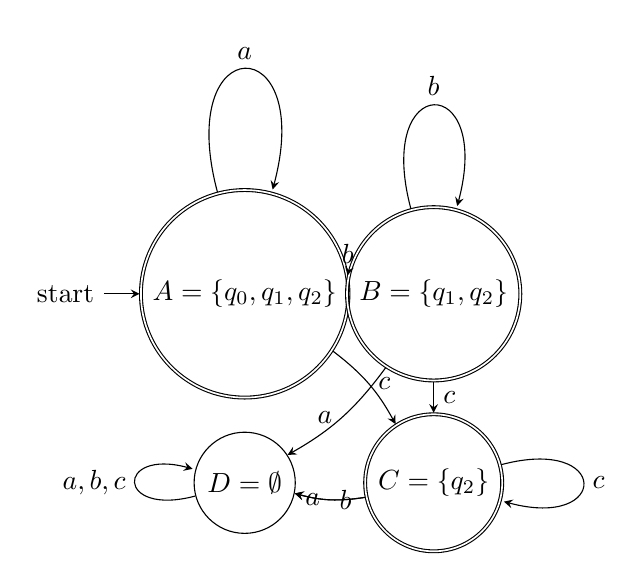
\begin{tikzpicture}[->,>=stealth,node distance=2.4cm,on grid,auto]
  \tikzstyle{every state}=[minimum size=1.2em]
  \node[state, initial, accepting]   (A) {$A=\{q_0,q_1,q_2\}$};
  \node[state, accepting, right=of A](B) {$B=\{q_1,q_2\}$};
  \node[state, accepting, below=of B](C) {$C=\{q_2\}$};
  \node[state, below=of A]           (D) {$D=\emptyset$};

  % A
  \path (A) edge[loop above] node{$a$} (A);
  \path (A) edge[bend left=12] node[above]{$b$} (B);
  \path (A) edge[bend left=12] node[right]{$c$} (C);

  % B
  \path (B) edge[loop above] node{$b$} (B);
  \path (B) edge[bend left=12] node[left] {$a$} (D);
  \path (B) edge node[right]{$c$} (C);

  % C
  \path (C) edge[loop right] node{$c$} (C);
  \path (C) edge[bend left=12] node[left] {$a$} (D);
  \path (C) edge[bend left=12] node[right]{$b$} (D);

  % D
  \path (D) edge[loop left] node{$a,b,c$} (D);
\end{tikzpicture}
\caption{Equivalent DFA $M_2'$ obtained by subset construction. States $A,B,C$ are accepting.}
\label{fig:dfa}
\end{figure}

\section{NFA Construction from Regular Expression $(00)^*(11)$}
We now convert the regular expression $r = (00)^*(11)$ into an NFA $M_3$ using Thompson's construction. The regex $r$ denotes the language
\[
L_3 = \{\,(00)^n\,11 \mid n \ge 0\}\,,
\]
i.e.\ any string consisting of some even number of \texttt{0}'s (including zero \texttt{0}'s) followed by \texttt{11}.

\medskip

\noindent \textbf{Thompson's Construction:} We build $M_3$ step by step:
\begin{enumerate}\itemsep0em
    \item For the sub-expression $00$: create an NFA with states $A$ (start) $\xrightarrow{0}$ $B$ $\xrightarrow{0}$ $C$ (final for this sub-NFA).
    \item Apply Kleene-* to $00$: introduce a new start state $I$ and new final state $F$. Add $\varepsilon$-transitions $I \xrightarrow{\varepsilon} A$ (enter the $00$ sub-NFA) and $I \xrightarrow{\varepsilon} F$ (to allow zero occurrences). Also add $\varepsilon$-transitions $C \xrightarrow{\varepsilon} A$ (to loop back after one occurrence) and $C \xrightarrow{\varepsilon} F$ (to exit after one or more occurrences). Now $I$ is the start and $F$ is the (temporary) final for $(00)^*$.
    \item For the sub-expression $11$: create an NFA with states $X$ (start) $\xrightarrow{1}$ $Y$ $\xrightarrow{1}$ $Z$ (final).
    \item Concatenate $(00)^*$ and $(11)$: connect the former's final to the latter's start by an $\varepsilon$-transition $F \xrightarrow{\varepsilon} X$. In the combined NFA, $I$ remains the initial state and $Z$ is the sole accepting state. (Note: $F$ is no longer an accepting state once concatenated, as a valid string must continue through the $11$ part.)
\end{enumerate}
Figure~\ref{fig:regex-nfa} shows the resulting NFA. State $I$ is the start and state $Z$ (double circle) is the accepting state.

\begin{figure}[h]\centering
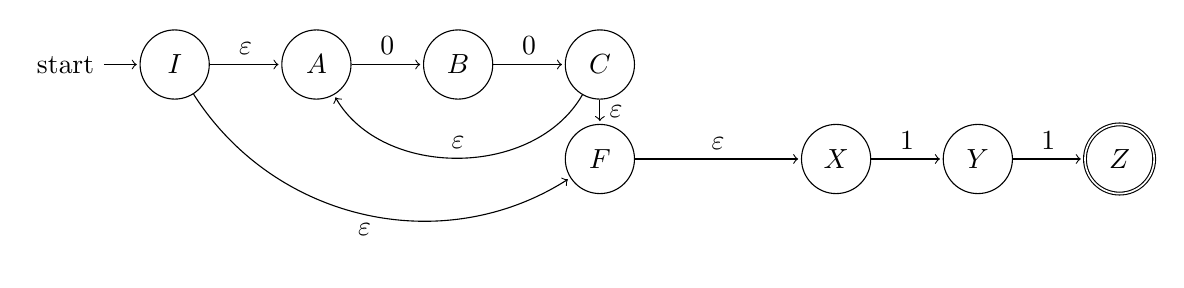
\begin{tikzpicture}[shorten >=1pt,node distance=1.8cm,on grid,auto]
    \node[state, initial] (I) {$I$};
    \node[state, right=of I] (A) {$A$};
    \node[state, right=of A] (B) {$B$};
    \node[state, right=of B] (C) {$C$};
    \node[state, below=1.2cm of C] (F) {$F$};
    \node[state, right=3cm of F] (X) {$X$};
    \node[state, right=of X] (Y) {$Y$};
    \node[state, accepting, right=of Y] (Z) {$Z$};
    % transitions for (00)* part
    \draw[->] (I) edge node[above] {$\varepsilon$} (A);
    \draw[->] (I) edge[bend right=45] node[below] {$\varepsilon$} (F);
    \draw[->] (A) edge node[above] {$0$} (B);
    \draw[->] (B) edge node[above] {$0$} (C);
    \draw[->] (C) edge[bend left=60] node[above] {$\varepsilon$} (A);
    \draw[->] (C) edge node[right] {$\varepsilon$} (F);
    % transitions for (11) part
    \draw[->] (F) edge node[above] {$\varepsilon$} (X);
    \draw[->] (X) edge node[above] {$1$} (Y);
    \draw[->] (Y) edge node[above] {$1$} (Z);
\end{tikzpicture}
\caption{NFA $M_3$ constructed for the regular expression $(00)^*(11)$.}
\label{fig:regex-nfa}
\end{figure}

To verify correctness: from $I$ to $F$, the machine can loop through $A \to B \to C$ any number of times, consuming pairs of \texttt{0}'s (each loop adds ``00'' to the string). The $\varepsilon$-transition $I \to F$ allows zero iterations of ``00''. After that, the $F \to X$ $\varepsilon$-move and the $X \to Y \to Z$ transitions consume \texttt{11}. Thus, the NFA accepts exactly those strings of the form $(00)^n 11$ for $n\ge0$, as required.

\section{Non-Regularity of $A_1 = \{www \mid w \in \{a,b\}^*\}$}
Finally, we prove that the language
\[
A_1 = \{\, w w w \mid w \in \{a,b\}^* \,\}
\]
is \emph{not} a regular language. Intuitively, $A_1$ consists of strings that can be divided into three equal parts, all identical. This is a classic example of a language that fails to meet the \textit{pumping lemma} criteria for regular languages. We provide a formal proof using the Pumping Lemma for regular languages.

\begin{theorem}
$A_1 = \{www \mid w \in \{a,b\}^*\}$ is not regular.
\end{theorem}
\begin{proof}
Suppose, for sake of contradiction, that $A_1$ is regular. Then by the Pumping Lemma, there exists a pumping length $p \ge 1$ such that any string $s \in A_1$ with $|s| \ge p$ can be decomposed as $s = x\,y\,z$, with $|xy| \le p$ and $|y| \ge 1$, and for all $i \ge 0$ the string $x\,y^i\,z$ is also in $A_1$.

Consider the specific string
\[
s = w\,w\,w \in A_1,\qquad \text{where } w = a^p b^p.
\]
Notice that $|w| = 2p$, so $|s| = 6p \ge p$. By construction, $s = a^p b^p\,a^p b^p\,a^p b^p$ (three copies of $w$). According to the lemma, $s$ can be written as $x y z$ with the stated properties. Since $|xy| \le p$, the substring $y$ lies entirely within the first $p$ characters of $s$. The first $p$ characters of $s$ are $a^p$ (all \texttt{a}). Thus, $y$ consists only of the letter \texttt{a}; say $y = a^k$ for some $k \ge 1$.

Now, consider pumping $y$ by taking $i=2$. The pumped string is:
\[
 s' \;=\; x\,y^2\,z \;=\; a^{p+k} b^p\,a^p b^p\,a^p b^p~,
\]
which has length $|s'| = 6p + k$.

If $A_1$ were regular, $s'$ must also belong to $A_1$. This means $s'$ should be expressible as $s' = t\,t\,t$ for some substring $t$. However, we will show this is impossible, leading to a contradiction:
\begin{itemize}\itemsep0em
    \item \textit{Length mismatch:} If $k$ is not a multiple of $3$, then $|s'| = 6p + k$ is not divisible by $3$. In that case, $s'$ cannot be split into three equal-length parts at all (let alone three identical parts), so $s' \notin A_1$.
    \item \textit{Content mismatch:} Suppose $k$ \textit{is} a multiple of $3$ (say $k=3m$) so that $|s'|$ is divisible by $3$. Then we can partition $s'$ into three substrings of equal length, each of length $2p + m$. However, these three substrings cannot all be equal. In $s'$, the first $2p+m$ characters (the first third of $s'$) include a longer prefix of \texttt{a}'s than the next $2p+m$ characters do. In fact, the first third of $s'$ starts with $a^{p+3m}$, whereas by the time we reach the beginning of the second third of $s'$, some of those \texttt{a}'s have been exhausted and replaced by \texttt{b}'s. Consequently, the second third of $s'$ begins with a different symbol than the first third does (it begins partway through the block of \texttt{b}'s), so the first and second segments of $s'$ are not identical. This means $s'$ is not of the form $t\,t\,t$.
\end{itemize}
In both cases, we reach a contradiction: $x y^2 z = s' \notin A_1$, despite $s \in A_1$. Therefore, our original assumption that $A_1$ is regular must be false. We conclude that $A_1$ is \textbf{not} a regular language.
\end{proof}

\end{document}
